\documentclass{weeklyreport}
\usepackage[utf8]{inputenc}

%%% Template Usage
% 1. Go to "All Projects" and make a copy in Overleaf,
% or download the source to modify locally.
% 2. Fill in your name
% 3. Set the reportdate to Monday of the current week


\title{Progress Report}
\author{Edris Qarghah}

\DTMsavedate{reportdate}{2020-07-06}
\date{Week of \DTMusedate{reportdate}}

\begin{document}

\maketitle

\newpage

\section*{Weekly Goals}

As this is the first week of my internship with Maniac Lab, my focus is on learning about the problems we are currently tackling and working out how I fit into the picture. A few broad categories:

\begin{itemize}
    \item Get access to the various systems/platforms used.
    \item Read documentation regarding the platforms we use.
    \item Review previous work done by members of the team and former interns.
    \item Explore the existing code-base.
    \item Study the topics underpinning our work (e.g., network tomography and anomaly detection)
    \item Develop a toy model so I can begin testing my understanding of these topics.
\end{itemize}

\section*{Daily Log}

\subsection*{\weekday{0}}

As this was the day before the internship began, I spent some time ensuring I was ready to hit the ground running.

\begin{itemize}
    \item Followed up with Rob about internship plans/preparations.
    \item \href{http://fasterdata.es.net/}{Read about ESNet}.
    \item Reviewed Time Series Analysis and Stochastic Modelling syllabus and supporting materials for references to anomaly detection.
    \item Gained access to \href{https://drive.google.com/drive/folders/1LlhbC0ow-dP2951RGwzURHQR_Z-0Le49?usp=sharing}{Google Drive folder}, \href{maniaclab.slack.com}{Maniac Lab Slack}, \href{https://github.com/maniaclab}{GitHub repo} and \href{https://docs.google.com/spreadsheets/d/10iPIfkq8TFPfNK93lgzEhBOzboEUTsx34XXU0fODKdk/edit?usp=sharing}{personal Google Drive folder}. 
    \item Reviewed \href{https://docs.google.com/document/d/1BDMqB2Bx64U3y_RKzZUxt2BklE5qFCcum5ZtTpWbBDA/edit?usp=sharing}{to-do list}.
\end{itemize}

\subsection*{\weekday{1}}

\begin{itemize}
    \item Met with Ilija to discuss Maniac Lab, the internship and related logistics.
    \item Got access to \href{https://atlas-kibana.mwt2.org:5601/}{ElasticSearch}, \href{https://drive.google.com/drive/folders/0APwP9-3JRjJOUk9PVA}{SAND Google Drive} and \href{https://codas.slateci.net/}{ML platform}.
    \item Set up Skype/Teams.
    \item \href{https://www.perfsonar.net/gtk_whatis.html}{Read about PerfSonar}.
    \item Gained access to \href{https://github.com/sand-ci}{SAND repo}.
    \item \href{https://drive.google.com/drive/folders/1ZzW0BQPzTr9K8w6xkqn9nV30oujFnreY?usp=sharing}{Read work by Suchant}.
    \item \href{https://www.overleaf.com/8647266712ttkyxfphmtvs}{Extended} Andrew's LaTeX document class and template for weekly reports to match template for \href{https://docs.google.com/presentation/d/1365SqaZjqrHnvYllhBcr7Z5zbP8dROKZKhFcWhOSFcE/edit?usp=sharing}{SAND presentations}.
    \item Created Google Sheets to track \href{https://docs.google.com/spreadsheets/d/1U9Ghphh7MsT3pbLcKU-PBj55ZeDankkhyYzn-XMLRMw/edit?usp=sharing}{contacts} and \href{https://docs.google.com/spreadsheets/d/10iPIfkq8TFPfNK93lgzEhBOzboEUTsx34XXU0fODKdk/edit?usp=sharing}{links to project materials/weekly reports.}
    \item Began \href{https://www.overleaf.com/2136625242fmfmybmnxbsh
}{first weekly report}.
    \item Spoke with Time Series professor who indicated he would try to work more anomaly detection related material into the course.
\end{itemize}

\subsection*{\weekday{2}}

\begin{itemize}
    \item Further extended \href{https://www.overleaf.com/8647266712ttkyxfphmtvs}{weekly report template} and updated \href{https://www.overleaf.com/2136625242fmfmybmnxbsh
}{this week's report}. 
    \item Read \href{https://netbeez.net/blog/network-tomography/}{several} \href{https://en.wikipedia.org/wiki/Network_tomography}{resources} on \href{https://www.cc.gatech.edu/~dovrolis/Courses/8803_F03/christos.pdf}{Network Tomography}.
    \item Read \href{https://www.oreilly.com/library/view/practical-time-series/9781492041641/ch04.html}{multiple} \href{https://adgefficiency.com/defaultdict/}{sources} about time series simulation in Python.
    \item Read overviews of \href{http://fasterdata.es.net/science-dmz/}{Science DMZ} and \href{http://fasterdata.es.net/network-tuning/tcp-issues-explained/}{TCP issues}.
    \item Explored ps\_packetloss data in Kibana to get a sense of what I'll be simulating.
    \item Read \href{https://towardsdatascience.com/anomaly-detection-with-time-series-forecasting-c34c6d04b24a}{several} \href{https://medium.com/pinterest-engineering/building-a-real-time-anomaly-detection-system-for-time-series-at-pinterest-a833e6856ddd}{sources} about anomaly detection in time series.
    \item Reviewed \href{http://egg.bu.edu/atlas/studies\%7btype:egg.Hatch\%7d/WAN-talk-SCW/WAN-4-ADC.pdf}{several} \href{http://egg.bu.edu/LHC\%7Binf:LHC\%7D/gadget:FTS/section:history/fts/docs/update-2015-06-09/FTS-update.pdf}{documents} from \href{http://egg.bu.edu/LHC\%7Binf:LHC\%7D/gadget:FTS/section:history/fts/index.htm}{Saul's old stuff}, though I'm not sure I got much value from it, as I don't think I have adequate context to understand what it is about.
    \item Initialized GitHub repo and installed Anaconda.
    \item Created \href{https://edrisq.codas.slateci.net/}{Jupyter Notebook} and tested functionality.
\end{itemize}

\subsection*{\weekday{3}}

\begin{itemize}
    \item Researched potential \href{https://www.grotto-networking.com/DiscreteEventPython.html}{methods} and tools for simulating network and time series data, such as \href{https://simpy.readthedocs.io/en/latest/}{SimPy}.
    \item Met with Ilija for clarification regarding toy problem and settled on the details for the project.
        \begin{itemize}
            \item Build a graph with the following features:
                \begin{itemize}
                    \item The graph has 100 nodes.
                    \item Each node is a coordinate on the $x,y$ plane.
                    \item Each node has a random number of connections (up to 4) to its nearest neighbors.
                    \item The edge/link connecting the nodes have a random bandwidth sampled from 10, 20, 40, 50, 80 and 100 Gbps.
                    \item The latency for each link is proportional to their geometric distance.
                \end{itemize}
            \item Simulate the network:
                \begin{itemize}
                    \item 10 random nodes are selected to "host" PerfSonar.
                    \item Initial simulation will have a single state, but later iterations will have packet flow that changes over time.
                \end{itemize}
            \item Create an observer that will make network measurements.
            \item Create a tool that will perform tomography on those measurements.
        \end{itemize}
    \item Learned of NetworkX from Andrew and read \href{https://networkx.github.io/documentation/stable/}{corresponding documentation}.
    \item Researched data-science project conventions and used \href{https://github.com/drivendata/cookiecutter-data-science}{cookiecutter project template} as described in \href{https://www.youtube.com/watch?v=HM56wCNxCnQ}{this video}.
    \item Created a graph\_test Jupyter notebook that creates a network that meets the minimum requirements discussed with Ilija and displays the network.
    \item Pushed project, including graph\_test notebook, license, requirements, etc.
    \item Configured \href{https://edrisq.codas.slateci.net/}{compute resource} to run the toy network files. 
\end{itemize}


\subsection*{\weekday{4}}

\begin{itemize}
    \item Completed Workday on-boarding tasks.
    \item Refactored network drawing into a separate function and added saving of figures.
    \item Created presentation for 2PM meeting.
    \item Read NetworkX documentation in search of a good method of ensuring trees are not disjoint (i.e, building an \href{https://networkx.github.io/documentation/stable/reference/algorithms/generated/networkx.algorithms.tree.mst.minimum_spanning_edges.html#networkx.algorithms.tree.mst.minimum_spanning_edges}{MST}).
    \item Set up \LaTeX locally, via \href{https://miktex.org/}{MiKTEX} and \href{https://www.xm1math.net/texmaker/}{Texmaker}, to facilitate pushing to GitHub without having to pay Overleaf.
    \item Completed weekly progress report and created corresponding makefile.
\end{itemize}

\section*{Achievements}
\subsection*{I learned about...}
\begin{itemize}
    \item ESNet
    \item PerfSonar
    \item Maniac Lab and SAND
    \item Network Tomography
    \item Anomaly Detection
    \item Science DMZ, common TCP issues
    \item NetworkX
    \item Cookiecutter Project template
    \item Jupyter notebooks
\end{itemize}

\pagebreak
\subsection*{I created...}
\begin{itemize}
	\item This progress report.
	\item A \href{https://docs.google.com/presentation/d/1Cm9z3TZmrk-BOiEYo0oock2HY4FlKp5m1iTx28EQzAQ/edit?usp=sharing}{presentation} for our weekly meeting.
    \item A \href{https://github.com/maniaclab/EdrisQarghah/tree/master/toy_network}{toy network} graph generator.
\end{itemize}

\begin{figure}[h!]
    \centering
    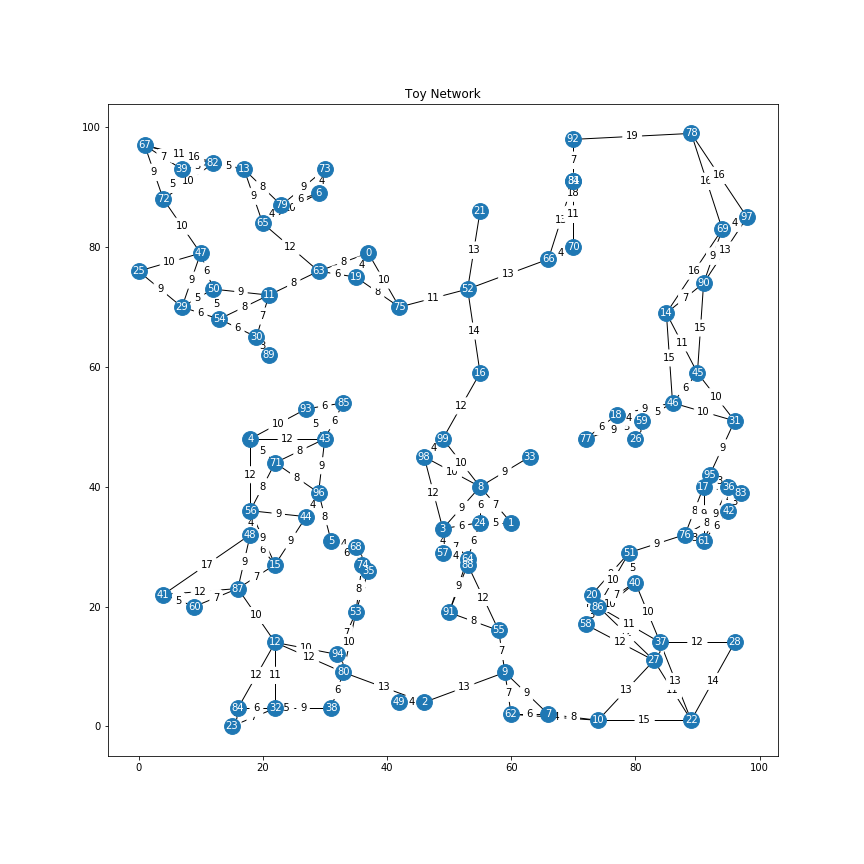
\includegraphics[width = \textwidth, trim = 85 90 85 85, clip]{week_1/Network_1a70e1d66f2040ce8a281f5823258bf1.png}
    \caption{An example of a network I generated.}
    \label{fig:Toy Network}
\end{figure}

\pagebreak
\section*{Roadblocks}
\subsection*{Questions}

\begin{itemize}
    \item What are good resources for network tomography?
    \item Are there good examples for me to use a template for my model?
    \item What is my title (for resume purposes)?
\end{itemize}

\subsection*{Problems}

Because the criteria for adding edges is to randomly add between 1 and 4 of the closest neighbors to a node, it is possible for a cluster of nodes to all have each other as their closest neighbors. This results in disjoint networks.

\begin{figure}[h!]
    \centering
    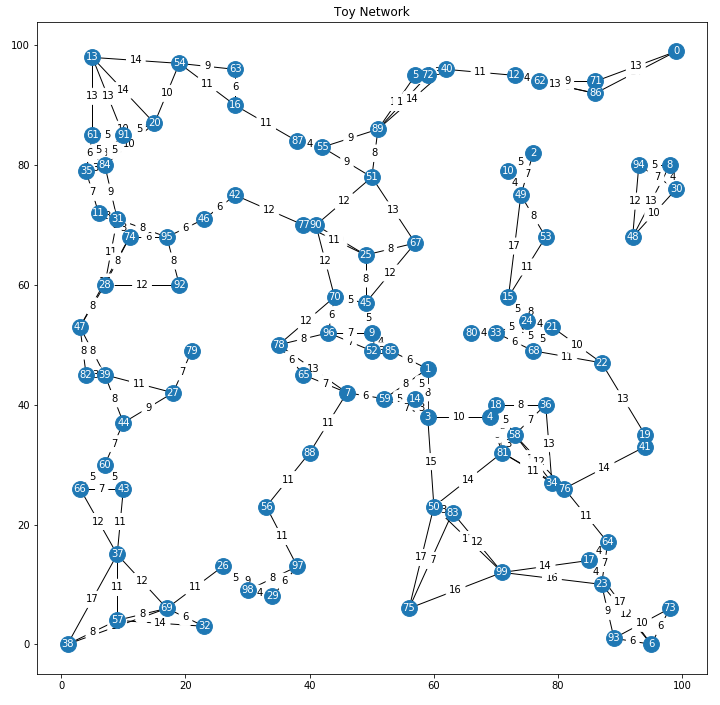
\includegraphics[width = \textwidth, trim = 85 90 85 85, clip]{week_1/Network_416b9f8671a64f04a87bbb59c431dc28.png}
    \caption{An example of disjoint networks generated.}
    \label{fig:Disjoint Networks}
\end{figure}

\subsection*{Challenges}

\begin{itemize}
    \item Displaying graphs on a plane
    \item Displaying node and edge details
\end{itemize}

\section*{Plans for Next Week}

\begin{itemize}
    \item Toy Network
    \begin{itemize}
        \item Create a more robust network generation process (e.g., ensuring MST).
        \item Simulate network activity.
        \item Measure activity from specific nodes and generate a resulting time series.
        \item Develop tools for tomography and anomaly detection.
        \item Improve visualization of networks.
    \end{itemize}
    \item Explore real network to understand how to better model it.
\end{itemize}

\end{document}
